\section{N-Gram Graph}

While writing this thesis we were searching for a good way to visualize the n-gram structure and distributions. What we came up with are the 

\begin{figure}[H]
	\minipage{1\textwidth}
	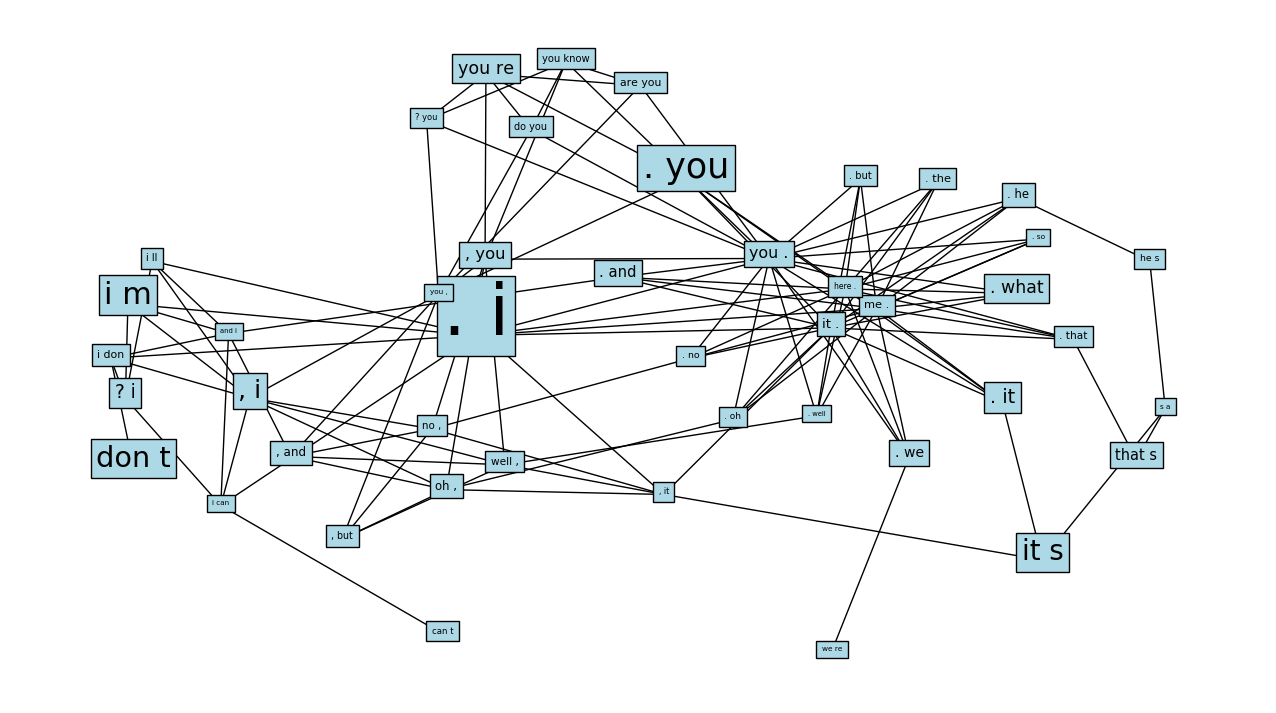
\includegraphics[width=\linewidth]{img/opensubtitles_bigram_top_50_graph}
	\centering
	\small
	\text{OpenSubtitles}
	\endminipage\hfill
	\minipage{1\textwidth}
	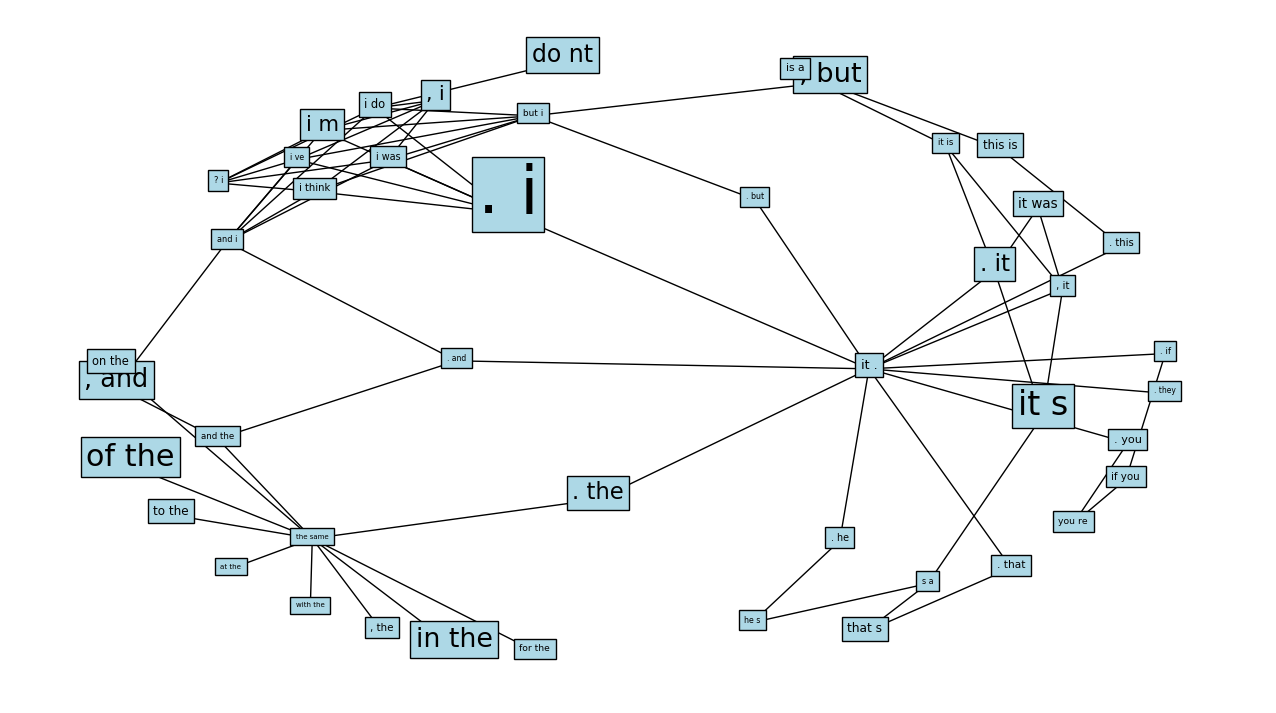
\includegraphics[width=\linewidth]{img/reddit_bigram_top_50_graph}
	\centering
	\small
	\text{Reddit}
	\endminipage\hfill
	\caption{N-Gram graphs for the 50 most used bigrams in the OpenSubtitles (upper) and Reddit (lower) datasets. Each node in the graphs represents a bigram, the edges between them show that either the first word of the first bigram matches the second word of the other bigram or the last word of the first bigram equals the last word of the second bigram. The size of each node is relative to its occurrence frequency, which means, that larger nodes occur more frequent than smaller ones.}
	\label{data:ngram:graph_top_50}
\end{figure}